\section{Experimental Evaluation}\label{section:experiments}

	We have implemented our solution as a modular client-server application in C++.
	We open-sourced all components of the software set: PathORAM~\cite{github-path-oram} and B+ tree~\cite{github-b-plus-tree} implementations and the main query executor~\cite{github-epsolute}.
	We provide PathORAM and B+ tree components as C++ libraries to be used in other projects; the code is documented, benchmarked and tested (228 tests covering \SI{100}{\percent} of the code).
	We have also published our datasets and query sets~\cite{our-datasets}.

	For cryptographic primitives, we used OpenSSL library (version 1.1.1i).
	For symmetric encryption in \acrshort{oram} we have used AES-CBC algorithm~\cite{nist-aes,nist-modes} with a 256-bits key (i.e., $\eta_2 = 2^{-256}$), for the hash algorithm \algo{H} used to partition records among \acrshortpl{oram} we have used SHA-256 algorithm~\cite{nist-hash}.
	Aggregate tree fanout \fanout{} is 16, proven to be optimal in~\cite{hierarchical-methods-for-dp}.

	We designed our experiments to answer the following questions:
	\newlength{\questionLength}
	\settowidth{\questionLength}{Question-5}
	\begin{description}[
		font=\bfseries,
		leftmargin=\dimexpr\questionLength+1.0em\relax,
		labelindent=0pt,
		labelwidth=\questionLength%
	]
		\item[Question-1\label{item:question-practicality}] How practical is our system compared to the most efficient and most private real-world solutions?
		\item[Question-2\label{item:question-storage}] How practical is the storage overhead?
		\item[Question-3\label{item:question-parameters}] How different inputs and parameters of the system affect its performance?
		\item[Question-4\label{item:question-scalability}] How well does the system scale?
		\item[Question-5\label{item:question-optimizations}] What improvements do our optimizations provide?
		\item[Question-6\label{item:question-attributes}] What is the impact of supporting multiple attributes?
	\end{description}

	To address \ref{item:question-practicality} we have run the default setting using conventional \acrshort{rdbms} (MySQL and PostgreSQL), Linear Scan approach and Shrinkwrap~\cite{shrinkwrap}. % chktex 2
	To target \ref{item:question-storage}, we measured the exact storage used by the client and the server for different data, record and domain sizes. % chktex 2
	To answer \ref{item:question-parameters}, we ran a default setting and then varied all parameters and inputs, one at a time. % chktex 2
	For \ref{item:question-scalability} we gradually added \acrshortpl{cpu}, \acrshort{oram} servers and \acrshort{kvs} instances and observed the rate of improvement in performance. % chktex 2
	For \ref{item:question-optimizations} we have run the default setting with our optimizations toggled. % chktex 2
	Lastly, for \ref{item:question-attributes} we have used two datasets to construct two indices and then queried each of the attributes. % chktex 2

	\subsection{Data sets}\label{section:experiments:data-sets}

		We used two real and one synthetic datasets --- California public pay pension database 2019~\cite{ca-employees-dataset} (referred to as ``CA employees''), Public Use Microdata Sample from US Census 2018~\cite{pums-dataset} (referred to as ``PUMS'') and synthetic uniform dataset.
		We have used salary / wages columns of the real datasets, and the numbers in the uniform set also represent salaries.
		The \texttt{NULL} and empty values were dropped.

		We created three versions of each dataset --- $10^5$, $10^6$ and $10^7$ records each.
		For uniform dataset, we simply generated the target number of entries.
		For PUMS dataset, we picked the states whose number of records most closely matches the target sizes (Louisiana for $10^5$, California for $10^6$ and the entire US for $10^7$).
		Uniform dataset was also generated for different domain sizes --- number of distinct values for the record.
		For CA employees dataset, the set contains \num{260 277} records, so we contracted it and expanded in the following way.
		For contraction we uniformly randomly sampled $10^5$ records.
		For expansion, we computed the histogram of the original dataset and sampled values uniformly within the bins.

		Each of the datasets has a number of corresponding query sets.
		Each query set has a selectivity or range size, and is sampled either uniformly or following the dataset distribution (using its \acrshort{cdf}).

	\subsection{Default setting}\label{section:experiments:default-setting}

		The default setting uses the \protocolGamma{} from \cref{section:prallel-dp-oram} and lightweight \acrshort{oram} machines from \cref{section:dp-improvements:three-tier,figure:three-tier}.
		We choose the \protocolGamma{} because it outperforms \protocolNoGamma{} in all experiments (see \textbf{\ref{item:question-scalability}} in \cref{section:experiments:results}).
		In the setting, there are 64 Redis services (8 services per one Redis server \acrshort{vm}), 8 \acrshort{oram} machines communicating with 8 Redis services each, and the client, which communicates with these 8 \acrshort{oram} machines.
		We have empirically found this configuration optimal for the compute nodes and network that we used in the experiments.
		\acrshort{oram} and Redis servers run on GCP \texttt{n1-standard-16} \acrshortpl{vm} (Ubuntu 18.04), in regions \texttt{us-east4} and \texttt{us-east1} respectively.
		Client machine runs \texttt{n1-highmem-16} \acrshort{vm} in the same region as \acrshort{oram} machines.
		The ping time between the regions (i.e.\ between trusted and untrusted zones) is \SI{12}{\milli\second} and the effective bandwidth is \SI{150}{\mega\byte\per\second}.
		Ping within a region is negligible.

		Default \acrshort{dp} parameters are $\epsilon = \ln(2) \approx \num{0.693}$ and $\beta = 2^{-20}$, which are consistent with the other \acrshort{dp} applications proposed in the literature~\cite{choosing-epsilon}.
		Buckets number is set as the largest power of $\fanout = 16$ that is no greater than the domain of the dataset \domainSize{}.

		Default dataset is a uniform dataset of $10^6$ records with domain size $10^4$, and uniformly sampled queries with selectivity \SI{0.5}{\percent}.
		Default record size is \SI{4}{\kibi\byte}.

	\subsection{Experiment stages}

		Each experiment includes running 100 queries such that the overhead is measured from loading query endpoints into memory to receiving the exact and whole query response from all \acrshort{oram} machines.
		The output of an experiment is, among other things, the overhead (in milliseconds), the number of real and noisy records fetched and communication volume averaged per query.

	\subsection{\acrshort{rdbms}, Linear Scan and Shrinkwrap}

		On top of varying the parameters, we have run similar workloads using alternative mechanisms --- extremes representing highest performance or highest privacy.
		Unless stated otherwise, the client and the server are in the trusted and untrusted regions respectively, with the network configuration as in \cref{section:experiments:default-setting}.

		\subsubsection*{Relational databases}

			Conventional \acrshort{rdbms} represents the most efficient and least private and secure solution in our set.
			While MySQL and PostgreSQL offer some encryption options and no differential privacy, for our experiments we turned off security features for maximal performance.
			We have run queries against MySQL and PostgreSQL varying data and record sizes.
			We used \texttt{n1-standard-32} GCP \acrshortpl{vm} in \texttt{us-east1} region, running MySQL version 14.14 and PostgreSQL version 10.14.

		\subsubsection*{Linear Scan}

			Linear scan is a primitive mechanism that keeps all records encrypted on the server then downloads, decrypts and scans the entire database to answer every query.
			This method is trivially correct, private and secure, albeit not very efficient.
			There are \acrshort{rdbms} solutions, which, when configured for maximum privacy, exhibit linear scan behavior (e.g., MS-SQL Always Encrypted with Randomized Encryption~\cite{mssql-always-enc} and Oracle Column Transparent Data Encryption~\cite{oracle-tde}).
			For a fair comparison we make the linear scan even more efficient by allowing it to download data via parallel threads matching the number of threads and bytes per request to that of our solution.
			Although linear scan is wasteful in the amount of data it downloads and processes, compared to our solution it has a benefit of not executing an \acrshort{oram} protocol with its logarithmic overhead and network communication in both directions.

		\subsubsection*{Shrinkwrap}

			Shrinkwrap~\cite{shrinkwrap} is a construction that answers federated \acrshort{sql} queries hiding both access pattern and communication volume.
			Using the EMP toolkit~\cite{emp-toolkit} and the code Shrinkwrap authors shared with us, we implemented a prototype that only answers range queries.
			This part of Shrinkwrap amounts to making a scan over the input marking the records satisfying the range, sorting the input, and then revealing the result set plus \acrshort{dp} noise to the client.
			For the latter part we have adapted Shrinkwrap's Truncated Laplace Mechanism~\cite[Definition 4]{shrinkwrap} to hierarchical method~\cite{hierarchical-methods-for-dp} in order to be able to answer an unbounded number of all possible range queries.
			We have emulated the outsourced database setting by using two \texttt{n1-standard-32} servers in different regions (\SI{12}{\milli\second} ping and \SI{150}{\mega\byte\per\second} bandwidth) executing the algorithm in a circuit model (the faster option per Shrinkwrap experiments) and then revealing the result to the trusted client.
			We note that although the complexity of a Shrinkwrap query is $\bigO{n \log n}$ due to the sorting step, its functionality is richer as it supports more relational operators, like \texttt{JOIN}, \texttt{GROUP BY} and aggregation.
			We also note that since MySQL, PostgreSQL and Shrinkwrap are not parallelized within the query, experiments using more \acrshortpl{cpu} do not yield higher performance.

	\subsection{Results and Observations}\label{section:experiments:results}

		After running the experiments, we have made the following observations.
		Note that we report results based on the default setting.
		\begin{itemize}[leftmargin=*]
			\item
				\epsolute{} is efficient compared to a strawman approach, \acrshort{rdbms} and Shrinkwrap: it is three orders of magnitude faster than Shrinkwrap, 18 times faster than the scan and only 4--8 times slower than a conventional database.
				In fact, for different queries, datasets, and record sizes, our system is much faster than the linear scan, as we show next.
			\item
				\epsolute{}'s client storage requirements are very practical: client size is just below \SI{30}{\mega\byte} while the size of the offloaded data is over 400 times larger.
			\item
				\epsolute{} scales predictably with the change in its parameters: data size affects performance logarithmically, record size --- linearly, and privacy budget $\epsilon$ --- exponentially.
			\item
				\epsolute{} is scalable: using \protocolGamma{} with the lightweight \acrshort{oram} machines, the increase in the number of threads translates into linear performance boost.
			\item
				The optimizations proposed in \cref{section:dp-improvements} provide up to an order of magnitude performance gain.
			\item
				\epsolute{} efficiently supports multiple indexed attributes.
				The overhead and the client storage increase slightly due to a lower privacy budget and extra local indices.
		\end{itemize}

		For the purposes of reproducibility we have put the log traces of all our experiments along with the instructions on how to run them on a publicly available page \href{https://epsolute.org}{epsolute.org}.
		Unless stated otherwise, the scale in the figures is linear and the $x$-axis is categorical.

		\subsubsection*{\textbf{\texorpdfstring{\ref{item:question-practicality}:}{} against \acrshort{rdbms}, Linear Scan and Shrinkwrap}}

			\begin{figure}[!ht]
	\centering
	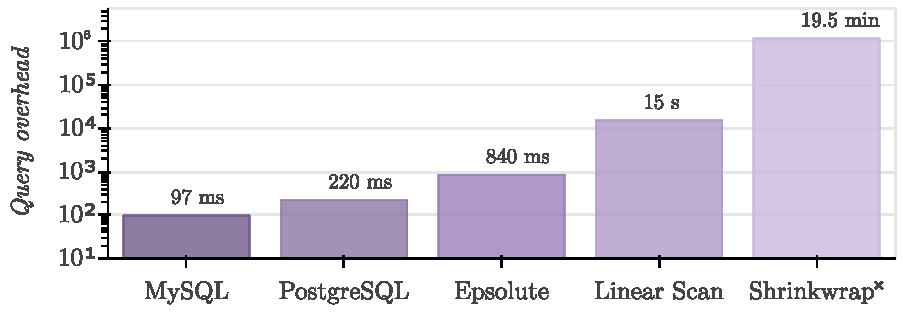
\includegraphics{mechanism}
	\caption[Different range-query mechanisms]{
		Different range-query mechanisms, logarithmic scale.
		Default setting: $10^6$ \SI{4}{\kibi\byte} uniformly-sampled records with the range $10^4$.
	}%
	\label{figure:mechanism}
\end{figure}


			The first experiment we have run using \epsolute{} is the default setting in which we observed the query overhead of \textbf{\SI[detect-all=true]{840}{\milli\second}}.
			To put this number in perspective, we compare \epsolute{} to conventional relational databases, the linear scan and Shrinkwrap.

			For the default setting, MySQL and PostgreSQL, configured for no privacy and maximum performance, complete in \SI{97}{\milli\second} and \SI{220}{\milli\second} respectively, which is just \textbf{8 to 4 times} faster than \epsolute{}, see \cref{figure:mechanism}.
			Conventional \acrshort{rdbms} uses efficient indices (B+ trees) to locate requested records and sends them over without noise and encryption, and it does so using less hardware resources.
			In our experiments \acrshort{rdbms} performance is linearly correlated with the result and record sizes.

			\begin{figure}[!ht]
	\centering
	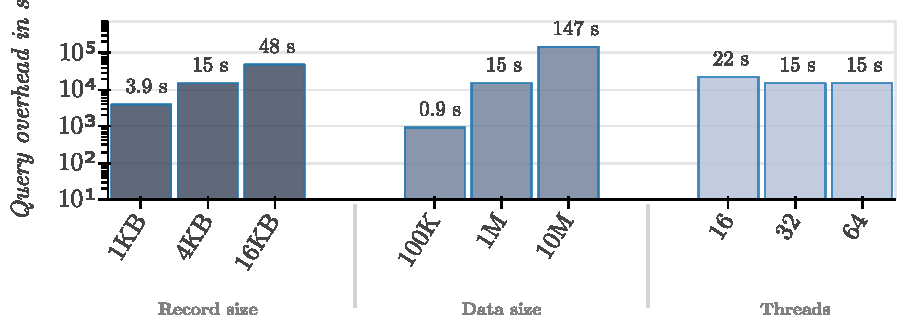
\includegraphics{linear-scan}
	\caption[Linear scan performance]{
		Linear scan performance, logarithmic scale.
		The experiments are run for the default setting of $10^6$ records of size \SI{4}{\kibi\byte} and 64 threads, with one of the three parameters varying.
	}%
	\label{figure:linear-scan}
\end{figure}


			Linear scan experiments demonstrate the practicality of \epsolute{} compared to a trivial ``download everything every time'' approach, see \cref{figure:linear-scan}.
			Linear scan's overhead is $\bigO{n}$ regardless of the queries, while \epsolute{}'s overhead is $\bigO{\log{n}}$ times the result size.
			According to our experiments, \epsolute{} eclipses the linear scan at \SI{4}{\kibi\byte}, 64 threads and only \emph{ten thousand records} (both mechanisms complete in about \SI{120}{\milli\second}).
			For a default setting (at a million records), the difference is \textbf{18 times}, see \cref{figure:linear-scan}.

			Because Shrinkwrap sorts the input obliviously in a circuit model, it incurs $\bigO{n \log n}$ comparisons, each resulting in multiple circuit gates, which is much more expensive than the linear scan.
			Unlike linear scan, however, Shrinkwrap does not require much client memory as the client merely coordinates the query.
			While Shrinkwrap supports richer set of relational operators, for range queries alone \epsolute{} is \textbf{three orders of magnitude} faster.

		\subsubsection*{\textbf{\texorpdfstring{\ref{item:question-storage}:}{} storage}}

			% chktex-file 26
% chktex-file 8

\newcommand{\lightvbar}{\color{lightGrey}\vrule}
\newcommand{\lightcline}[1]{\arrayrulecolor{lightGrey}\cline{#1}\arrayrulecolor{black}}

\begin{table}[!ht]
	\renewcommand{\arraystretch}{1.2}
	\sisetup{detect-all = true}
	\begin{tabular*}{\linewidth}{ !{\extracolsep\fill} c | r !{\lightvbar{}} r | r !{\lightvbar{}} r | r !{\lightvbar{}} r} % chktex 44
		\toprule
			\diagbox{\dataSize}{\scriptsize{Record}}			& \multicolumn{2}{c !{\lightvbar{}}}{\SI{1}{\kibi\byte}}				& \multicolumn{2}{c !{\lightvbar{}}}{\SI{4}{\kibi\byte}}				& \multicolumn{2}{c}{\SI{16}{\kibi\byte}}												\\
		\midrule
			\multirow{2}{*}{$10^5$}								& \small\SI{400}{\kibi\byte}			& \small\SI{400}{\byte}			& \small\SI{400}{\kibi\byte}			& \small\SI{102}{\kibi\byte}	& \small\SI{400}{\kibi\byte}					& \small\SI{1.6}{\mega\byte}			\\ \lightcline{2-3} \lightcline{4-5} \lightcline{6-7}
																& \small\bfseries\SI{396}{\mega\byte}	& \small\SI{4.6}{\mega\byte}	& \small\bfseries\SI{1.5}{\giga\byte}	& \small\SI{14}{\mega\byte}		& \small\bfseries\SI{6.2}{\giga\byte}			& \small\SI{51}{\mega\byte}				\\

		\midrule
			\multirow{2}{*}{$10^6$}								& \small\SI{3.9}{\mega\byte}			& \small\SI{400}{\byte}			& \small\SI{3.9}{\mega\byte}			& \small\SI{102}{\kibi\byte}	& \small\SI{3.9}{\mega\byte}					& \small\SI{1.6}{\mega\byte}			\\ \lightcline{2-3} \lightcline{4-5} \lightcline{6-7}
																& \small\bfseries\SI{3.2}{\giga\byte}	& \small\SI{15}{\mega\byte}		& \small\bfseries\SI{12}{\giga\byte}	& \small\SI{25}{\mega\byte}		& \small\bfseries\SI{48}{\giga\byte}			& \small\SI{62}{\mega\byte}				\\

		\midrule
			\multirow{2}{*}{$10^7$}								& \small\SI{40}{\mega\byte}				& \small\SI{400}{\byte}			& \small\SI{40}{\mega\byte}				& \small\SI{102}{\kibi\byte}	& \small\itshape\SI{40}{\mega\byte}				& \small\itshape\SI{1.6}{\mega\byte}	\\ \lightcline{2-3} \lightcline{4-5} \lightcline{6-7}
																& \small\bfseries\SI{24}{\giga\byte}	& \small\SI{99}{\mega\byte}		& \small\bfseries\SI{96}{\giga\byte}	& \small\SI{109}{\mega\byte}	& \small\itshape\bfseries\SI{384}{\giga\byte}	& \small\itshape\SI{146}{\mega\byte}	\\

		\midrule
			\diagbox[dir=SW, width=6em]{\dataSize}{\domainSize}	& \multicolumn{2}{c !{\lightvbar{}}}{$100$}								& \multicolumn{2}{c !{\lightvbar{}}}{$10^4$}							& \multicolumn{2}{c}{$10^6$}															\\
		\toprule
	\end{tabular*}
	\sisetup{detect-none = true}
	\caption[Storage usage for varying data, record and domain sizes]{
		Storage usage for varying data, record and domain sizes.
		The values are as follows.
		Left top: index \indexI{} (B+ tree), right top: aggregate tree \serverDS{}, right bottom: \acrshort{oram} \user{} state and left bottom (bold): \acrshort{oram} \server{} state.
		\textit{Italic} indicates that the value is estimated.
	}%
	\label{table:storage}
\end{table}


			While \epsolute{} storage efficiency is near-optimal \efficiency{1}{0}, it is important to observe the absolute values.
			Index \indexI{} is implemented as a B+ tree with fanout 200 and occupancy \SI{70}{\percent}, and its size, therefore, is roughly $5.7 \dataSize$ bytes.
			Most of the \acrshort{oram} client storage is the PathORAM stash with its size chosen in a way to bound failure probability to about $\eta_1 = 2^{-32}$ (see \cite[Theorem 1]{path-oram}). % chktex 2
			In \cref{table:storage}, we present \epsolute{} storage usage for the parameters that affect it --- data, record and domain sizes.
			We measured the sizes of the index \indexI{}, \acrshort{dp} structure \serverDS{}, and \acrshort{oram} client and server states.
			Our observations are:
			\begin{enumerate*}[label={(\roman*)}]
				\item index size expectedly grows only with the data size,
				\item \serverDS{} is negligibly small in practice,
				\item small \indexI{} and \serverDS{} sizes imply the efficiency of supporting multiple indexed attributes,
				\item \server{} to \user{} storage size ratio varies from \textbf{85} in the smallest setting to more than \textbf{\num[detect-all=true]{2000}} in the largest, and
				\item one can trade client storage for \acrshort{oram} failure probability.
			\end{enumerate*}
			We conclude that the storage requirements of \epsolute{} are practical.

			% Stash size calculations are based on stash size 49, which, according to PathORAM paper, results in 14*0.6^{49} = 2^{-32} probability of failure

			% Total ORAM client size (in MB) is (( (2^h * 3 +3)*4 ) + (49 * (r * 1024) + 16))*64 / 1024^2
			% where h is ORAM_LOG_CAPACITY (11, 14, 17) and r is the record size in the number of kilobytes (1, 4, 16)

		\subsubsection*{\textbf{\texorpdfstring{\ref{item:question-parameters}:}{} varying parameters}}

			\begin{figure}[!ht]
	\centering
	\begin{minipage}{0.48\textwidth}
		\centering
		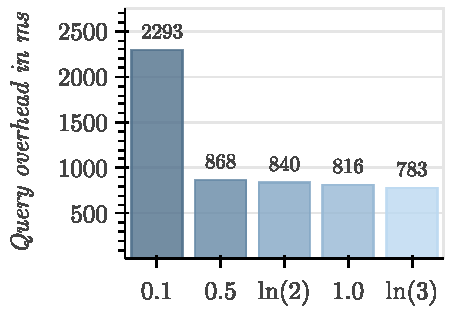
\includegraphics[width=\linewidth]{epsilon}
		\captionof{figure}{Privacy budget $\epsilon$}%
		\label{figure:epsilon}
	\end{minipage}
	~ % chktex 39
	\begin{minipage}{0.48\textwidth}
		\centering
		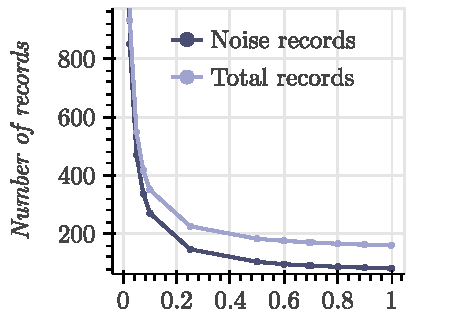
\includegraphics[width=\linewidth]{epsilon-effect}
		\captionof{figure}{Effect of $\epsilon$}%
		\label{figure:epsilon-effect}
	\end{minipage}
\end{figure}


			To measure and understand the impact of configuration parameters on the performance of our solution we have varied $\epsilon$, record size, data size \dataSize{}, domain size \domainSize{}, selectivities, as well as data and query distributions.
			The relation that is persistent throughout the experiments is that for given data and record sizes, the performance (the time to completely execute a query) is strictly proportional to the total number of records, fake and real, that are being accessed per query.
			Each record access goes through the \acrshort{oram} protocol, which, in turn, downloads, re-encrypts and uploads $\bigO{\log{\dataSize}}$ blocks.
			These accesses contribute the most to the overhead and all other stages (e.g., traversing index or aggregate tree) are negligible.

			\paragraph*{Privacy budget \texorpdfstring{$\epsilon$}{epsilon} and its effect}

				We have run the default setting for $\epsilon = \{ 0.1, \allowbreak 0.5, \allowbreak \ln{2}, \allowbreak 1.0, \allowbreak \ln{3} \}$.
				$\epsilon$ strictly contributes to the amount of noise, which grows exponentially as $\epsilon$ decreases, see \cref{figure:epsilon}, observe sharp drop.
				As visualized on \cref{figure:epsilon-effect}, at high $\epsilon$ values the noise contributes a fraction of total overhead, while at low values the noise dominates the overhead entirely.

			\begin{figure}[!ht]
	\centering
	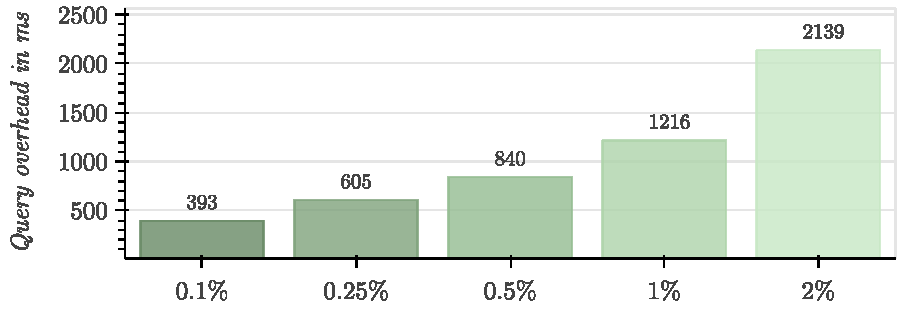
\includegraphics[width=\linewidth]{selectivity}
	\caption{Selectivity}%
	\label{figure:selectivity}
\end{figure}


			\paragraph*{Selectivity}

				We have ranged the selectivity from \SI{0.1}{\percent} to \SI{2}{\percent} of the total number of records, see \cref{figure:selectivity}.
				Overhead expectedly grows with the result size.
				For smaller queries, and thus for lower overhead, the relation is positive, but not strictly proportional.
				This phenomena, observed for the experiments with low resulting per-query time, is explained by the variance among parallel threads.
				During each query the work is parallelized over \oramsNumber{} \acrshortpl{oram} and the query is completed when the \emph{last} thread finishes.
				The problem, in distributed systems known as ``the curse of the last reducer''~\cite{curse-of-last-reducer}, is when one thread takes disproportionally long to finish.
				In our case, we run 64 threads in default setting, and the delay is usually caused by a variety of factors --- blocking \acrshort{io}, network delay or something else running on a shared virtual \acrshort{cpu}.
				This effect is noticeable when a single thread does relatively little work and small disruptions actually matter; the effect is negligible for large queries.

			\begin{figure}[!ht]
	\centering
	\begin{minipage}{0.31\columnwidth}
		\centering
		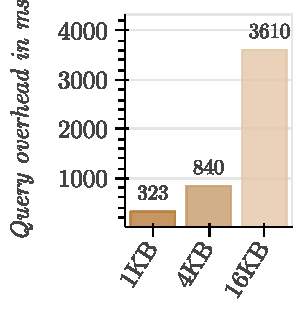
\includegraphics[width=\linewidth]{record-size}
		\captionof{figure}{Record size}%
		\label{figure:record-size}
	\end{minipage}
	~ % chktex 39
	\begin{minipage}{0.31\columnwidth}
		\centering
		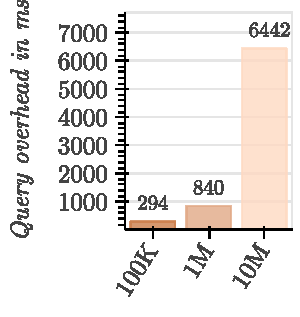
\includegraphics[width=\linewidth]{data-size}
		\captionof{figure}{Data size}%
		\label{figure:data-size}
	\end{minipage}
	~ % chktex 39
	\begin{minipage}{0.31\columnwidth}
		\centering
		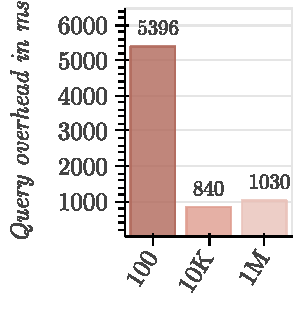
\includegraphics[width=\linewidth]{domain-size}
		\captionof{figure}{Domain size}%
		\label{figure:domain-size}
	\end{minipage}
\end{figure}


			\paragraph*{Record, data and domain sizes}

				We have tried \SI{1}{\kibi\byte}, \SI{4}{\kibi\byte} and \SI{16}{\kibi\byte} records, see \cref{figure:record-size}.
				Trivially, the elapsed time is directly proportional to the record size.

				We set \dataSize{} to $10^5$, $10^6$ and $10^7$, see \cref{figure:data-size}.
				The observed correlation of overhead against the data size is positive but non-linear, 10 times increment in \dataSize{} results in less than 10 times increase in time.
				This is explained by the \acrshort{oram} overhead --- when \dataSize{} changes, the \acrshort{oram} storage gets bigger and its overhead is logarithmic.

				For synthetic datasets we have set \domainSize{} to $100$, $10^4$ and $10^6$, see \cref{figure:domain-size}.
				The results for domain size correlation are more interesting: low and high values deliver worse performance than the middle value.
				Small domain for a large data set means that a query often results in a high number of real records, which implies significant latency regardless of noise parameters.
				A sparse dataset, on the other hand, means that for a given selectivity wider domain is covered per query, resulting in more nodes in the aggregate tree contributing to the total noise value.

			\begin{figure}[!ht]
	\centering
	\begin{minipage}{0.48\columnwidth}
		\centering
		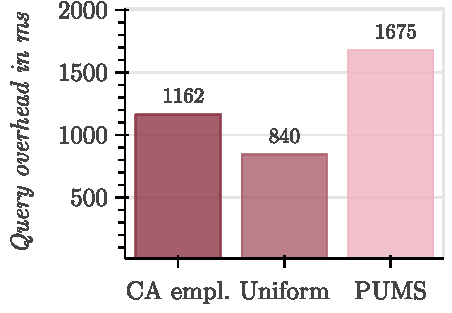
\includegraphics{data-distribution}
		\captionof{figure}{Data distribution}%
		\label{figure:data-distribution}
	\end{minipage}
	~ % chktex 39
	\begin{minipage}{0.48\columnwidth}
		\centering
		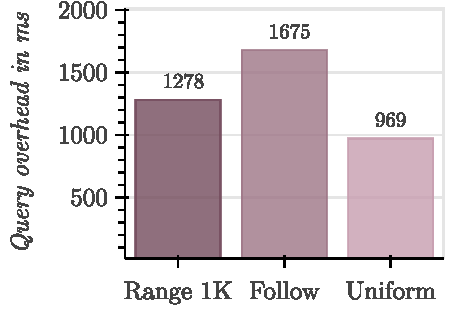
\includegraphics{query-distribution}
		\captionof{figure}{Query distribution}%
		\label{figure:query-distribution}
	\end{minipage}
\end{figure}


			\paragraph*{Data and query distributions}

				Our solution performs best on the uniform data and uniform ranges, see \cref{figure:data-distribution,figure:query-distribution}.
				Once a skew of any kind is introduced, there appear sparse and dense regions that contribute more overhead than uniform regions.
				Sparse regions span over wider range for a given selectivity, which results in more noise.
				Dense regions are likely to include more records for a given range size, which again results in more fetched records.
				Both real datasets are heavily skewed towards smaller values as few people have ultra-high salaries.

		\subsubsection*{\textbf{\texorpdfstring{\ref{item:question-scalability}:}{} scalability}}

			\begin{figure}[th]
	\centering
	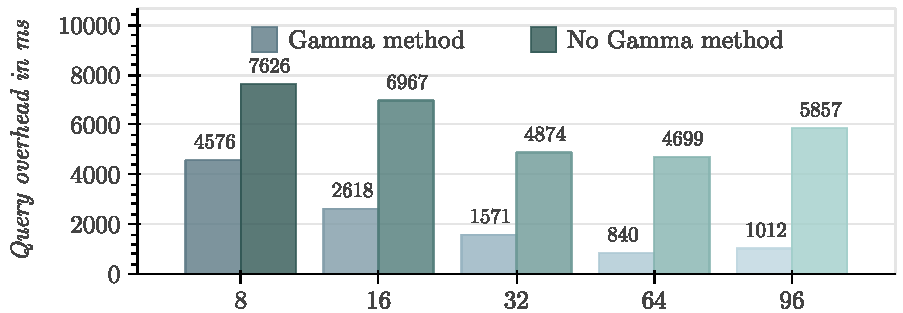
\includegraphics[width=\textwidth]{scalability}
	\caption[Scalability measurements for different methods of noise generation]{
		Scalability measurements for shared \serverDS{} structure \protocolGamma{} and separate \serverDS{} structures \protocolNoGamma{}
	}%
	\label{figure:scalability}
\end{figure}


			Horizontal scaling is a necessity for a practical system, this is the motivation for the parallelization in the first place.
			Ideally, performance should improve proportionally to the parallelization factor, number of \acrshortpl{oram} in our case, \oramsNumber{}.

			For scalability experiments we run the default setting for both \protocolNoGamma{} and \protocolGamma{} (\emph{no-$\gamma$-method} and \emph{$\gamma$-method} respectively) varying the number of \acrshortpl{oram} \oramsNumber{}, from 8 to 96 (maximum virtual \acrshortpl{cpu} on a GCP \acrshort{vm}).
			The results are visualized on \cref{figure:scalability}.
			We report two positive observations:
			\begin{enumerate*}[label={(\roman*)}]
				\item the $\gamma$-method provides substantially better performance and storage efficiency, and
				\item when using this method the system scales linearly with the number of \acrshortpl{oram}.
			\end{enumerate*}
			($\oramsNumber = 96$ is a special case because some \acrshortpl{oram} had to share a single \acrshort{kvs}.)

		\subsubsection*{\textbf{\texorpdfstring{\ref{item:question-optimizations}:}{} optimizations benefits}}

			\begin{table}[!ht]
	\begin{tabular*}{\linewidth}{ !{\extracolsep\fill} l c c >{\bfseries}c } % chktex 26
		\toprule
			Improvement (section)													& Enabled					& Disabled					& Boost			\\
		\midrule
			\acrshort{oram} batching (\ref{section:dp-improvements:oram-batching})				& \SI{840}{\milli\second}	& \SI{6978}{\milli\second}	& 8.3x			\\
			Lightweight \acrshort{oram} machines (\ref{section:dp-improvements:three-tier})	& \SI{840}{\milli\second}	& \SI{4484}{\milli\second}	& 5.3x			\\
			Both improvements														& \SI{840}{\milli\second}	& \SI{8417}{\milli\second}	& \emph{10.0x}	\\
		\bottomrule
	\end{tabular*}
	\caption{Improvements over parallel \epsolute{}}%
	\label{table:optimizations}
\end{table}


			\cref{table:optimizations} demonstrates the boosts our improvements provide; when combined, the speedup is up to an order of magnitude.

			\acrshort{oram} request batching (\cref{section:dp-improvements:oram-batching}) makes the biggest difference.
			We have run the default setting with and without the batching.
			The overhead is substantially smaller because far fewer \acrshort{io} requests are being made, which implies benefits across the full stack: download, re-encryption and upload.

			Using lightweight \acrshort{oram} machines (\cref{section:dp-improvements:three-tier}) makes a difference when scaling.
			In the default setting, 64 parallel threads quickly saturate the memory access and network channel, while spreading computation among nodes removes the bottleneck.

		\subsubsection*{\textbf{\texorpdfstring{\ref{item:question-attributes}:}{} multiple attributes}}

			\begin{figure}[!ht]
	\centering
	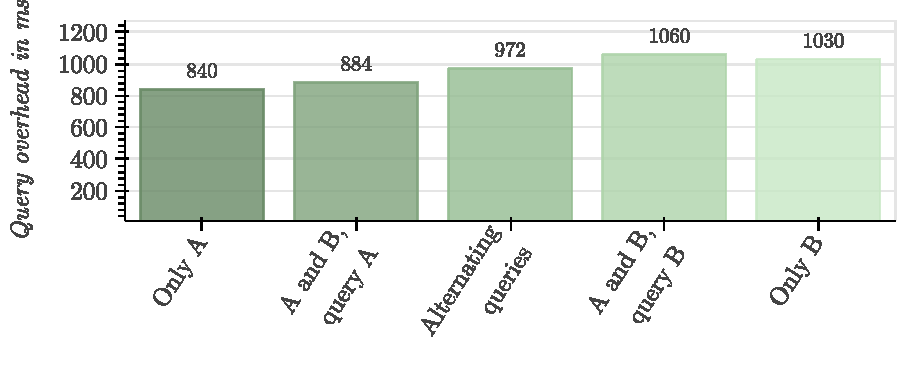
\includegraphics[width=\columnwidth]{multiple-attributes}
	\caption[Query overhead when using multiple attributes]{
		Query overhead when using multiple attributes.
		\emph{Only A} and \emph{Only B} index one attribute.
		\emph{A and B} indexes both attributes and then queries one of them.
		\emph{Alternating} indexes both attributes and runs half of the queries against \emph{A} and another half against \emph{B}.
	}%
	\label{figure:attributes}
\end{figure}


			\epsolute{} supports multiple indexed attributes.
			In \cref{section:dp-oram:multiple-attributes} we described that the performance implications amount to having an index \indexI{} and a \acrshort{dp} structure \serverDS{} per attribute and sharing the privacy budget $\epsilon$ among all attributes.
			As shown in \cref{table:storage}, \indexI{} and \serverDS{} are the smallest components of the client storage.
			To observe the query performance impact, we have used the default dataset with domains $10^4$ and $10^6$ as indexed attributes \emph{A} and \emph{B} respectively.
			We ran queries against only \emph{A}, only \emph{B} and against both attributes in alternating fashion.
			Each of the attributes used $\epsilon = \frac{\ln{2}}{2}$ to match the default privacy budget of $\ln(2)$.

			\cref{figure:attributes} demonstrates the query overhead of supporting multiple attributes.
			The principal observation is that the overhead increases only slightly due to a lower privacy budget.
			The client storage went up by just \SI{9}{\mega\byte}, and still constitutes only \SI{3.3}{\percent} of the server storage, which is not affected by the number of indexed attributes.

			% for 10K domain: total client storage went from 3.9+0.1+25 to 3.9+0.1+25+9, i.e. 31%
			% for 1M domain: total client storage went from 3.9+1.6+25 to 3.9+1.6+25+9, i.e. 29.5%
